%%This is a very basic article template.
%%There is just one section and two subsections.
\documentclass[parskip=full]{scrartcl}
\usepackage[table]{xcolor}

\usepackage{amsmath}
\usepackage{amsfonts}
\usepackage{mathtools}
\usepackage{studarbeit}
\usepackage{graphicx}
\usepackage{wrapfig}
\usepackage{lscape}
\usepackage{rotating}
\usepackage{epstopdf}
\usepackage{pdfpages}
\usepackage{caption, booktabs}
\usepackage{tabularx}
\usepackage{multirow}
\usepackage[binary-units=true]{siunitx}
 \usepackage[autostyle=true,german=quotes]{csquotes}
 \usepackage{longtable, booktabs}
 \newcommand{\swtLabel}[1]{\textbf{/#1\arabic*0/}}
 \begin{document}

\title{Elipse -- Einteilungs Interface für das PSE}
\author{D. Biester, E. Dohse, P. Faller, P. Loth, L. Seufert, S. Kopmann}
\thesistype{Implementierungsdokument}
\zweitgutachter{}
\betreuer{Dipl.-Inform.~Andreas~Zwinkau, M.Sc.~Andreas~Fried}
\coverimage{ElipseLogo.png}
\mytitlepage
{\setlength{\textheight}{297mm}
\tableofcontents

\setlength{\textheight}{297mm}}
\pagebreak

\section{Einleitung}
Nach dem im Pflichtenheft beschrieben wurde, was das Produkt leisten soll und
das Entwurfsdokument beantwortete  wie das Produkt strukturert sein soll, beschreibt dieses Dokument nun die Implementierung also die Umsetzung der beiden vorherigen Dokumente. 

\section{Implementierungsplan}
Zu beginn der Implementierungsphase wurde ein Plan erstellt, der unser
vorgesehenes Vorgehen beschreibt.
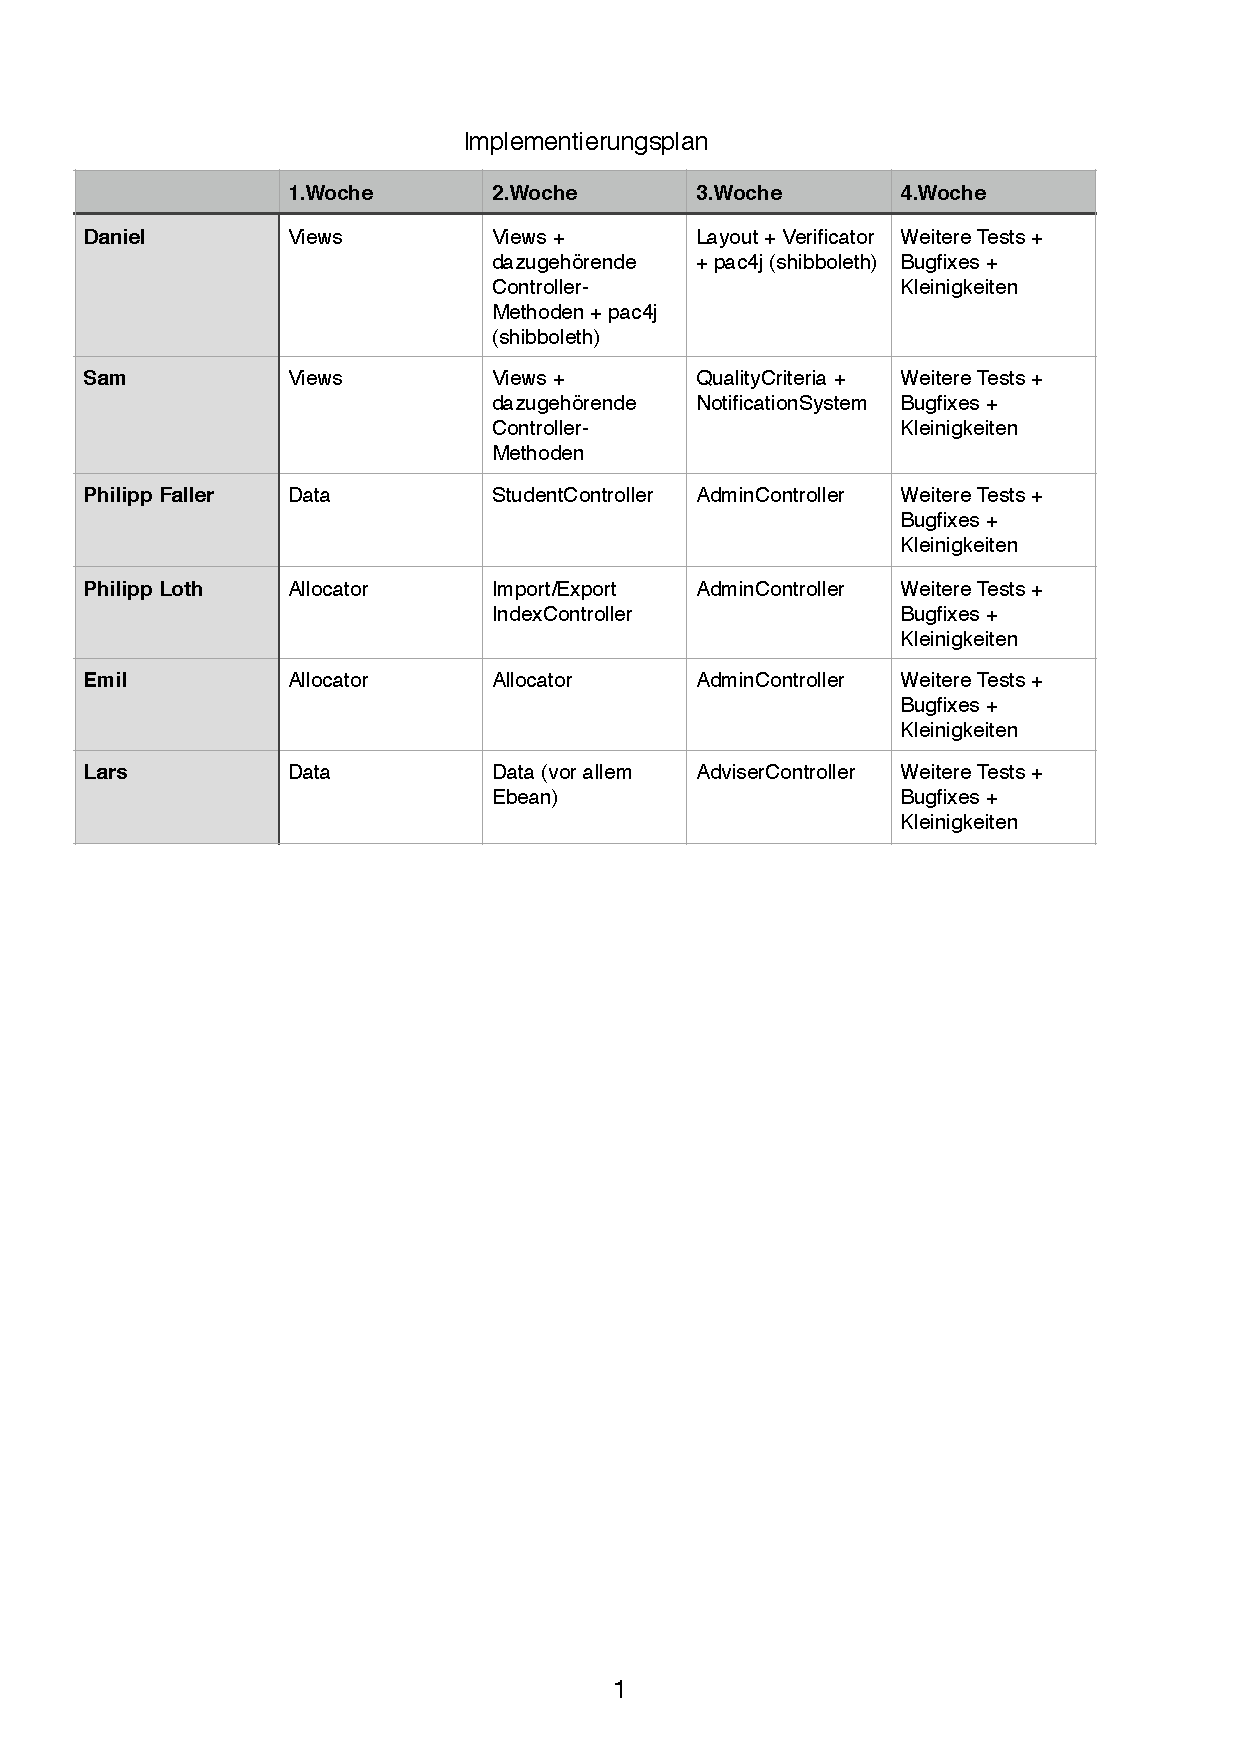
\includepdf[pages={1}]{Implementierungsplan.pdf}
\begin{table}
\begin{tabularx}{\textwidth}{p{0.175\textwidth}|X|X|X|X|}
 	& 1. Woche			& 2. Woche		& 3. Woche & 4. Woche\\
\hline \hline
Daniel	& Views			& Views + dazugehörige Controller-Methoden + pac4j 
(shibboleth) & Layout + Verificator
+ pac4j (shibboleth)& Weitere Tests +
Bugfixes +
Kleinigkeiten\\
\hline
Sam & Views&Views +
dazugehörende
Controller-
Methoden & QualityCriteria +
NotificationSystem & Weitere Tests +
Bugfixes +
Kleinigkeiten\\
\hline
Philipp Faller&Data&Import/Export
IndexController&AdminController&Weitere Tests +
Bugfixes +
Kleinigkeiten\\
\hline
Emil&Allocator&Allocator&AdminController&Weitere Tests +
Bugfixes +
Kleinigkeiten\\
\hline
Lars&Data&Data (vor allem
Ebean)&AdviserController&Weitere Tests +
Bugfixes +
Kleinigkeiten\\
\hline
\end{tabularx}
\end{table}
% Hierbei war der für uns \enquote{kritische Pfad} %TODO Was ist unser Criticall
% % Path 
% das das Datenmodell gefolgt von paralell implementierbaren Controllern die nur
% auf das Datenmodell zugreiffen und der Allocation. 
Mit sechs Entwicklern in der kurzen Zeit von nur 4 Wochen, die auch noch in der
Prüfungsphase liegt, ein Software-Produkt zu implementieren erfordert, dass die
Entwickler effizient arbeiten können. Da sich jeder von uns bereits in der
Entwurfsphase auf ein Gebiet spezialisiert hatte bot es sich an jedem auf seinem
Fachgebiet auch die Implementierung zu übertragen. 
Ein weiterer Grund für unser Vorgehen war, das wir den Aufwand für
Web-Entwicklung, also das implementieren der Views und deren Anbindung an
die Controller und das verwenden von ORM-Tools nicht einschätzen konnten. Daher
wollten wir hier frühzeitig ein funktionierendes Grundgerüst schaffen.
Genau diese herangehensweise bewährte sich, da die Arbeit mit eBean (unserem
ORM-Tool) und dem Play-Framework sich als weit anstrengender herausstellte als
gedacht. Veraltete und nicht vorhandene Dokumentatonen, leer implementerte
Methoden und den guten Ratschlag bei StackOverflow die doch
lieber Hibernate zu verwenden - alltäglich.


Bei der 
%TODO zweites Diagramm wie haben wir wirklich implementeirt

%dann fairness bzw hierzu nur einen satz aber allgemeine statistiken 
%
\section{Änderungen zum Entwurfsdokument}
Zur Sicherung bessere Code-Qualität (z.B. dem Vermeiden von Code-Copy-Pasting)
und maßgeblich durch die oben beschriebenen Probleme mit verschiedenen
verwendeten Bibliotheken  wurden Änderungen im Vergleich zum  Entrurfsdokument
vorgenommen:
\begin{itemize}
  \item 
\end{itemize}

\section{Funktionsumfang}
Wie im Pflichtenheft beschrieben gibt es einige Muss und Wunschkriterien zu
diesem Produkt. Ein Großteil dieser wurde von uns Implementiert.
\subsection{Einteilungsfunktionen}
\subsubsection{Pflichtfunktionen}
\begin{enumerate}[label=\swtLabel{FA}]
  \item Einteilung der Studierenden zu Projekten. Hierbei werden folgende Kriterien,
soweit möglich und wie konfiguriert berücksichtigt:
\begin{itemize}
  \item Wer die durch seine SPO gegebenen Voraussetzungen nicht erfüllt, wird nicht
eingeteilt
\item Möglichst viele Studierende werden zu Projekten zugeteilt
\item Lerngruppen bleiben zusammen
\item Projektbewertung der Studierenden werden berücksichtigt
\end{itemize}
\item Berechnung von Gütekriterien
\end{enumerate}
\subsubsection{Wunschfunktionen}
\begin{enumerate}[label=\swtLabel{FA}, resume]
  \item Stapelverarbeitung von mehreren Einteilungen mit unterschiedlichen Konfigurationen
\item Folgende Kriterien fließen in die Einteilung ein:
\begin{itemize}
  \item Wer sich zum zweiten Mal bewirbt, soll bei der Einteilung bevorzugt
  werden
  \item Eher 5er-Teams als 6er-Teams
  \item Studierende in einem Team sind im gleichen Semester
  \item Studierende höheren Semesters werden bevorzugt
  \item Studierende, die bereits mehr Teilleistungen aus dem ersten Jahr bestanden
haben, werden bevorzugt
\end{itemize}
\end{enumerate}
\subsection{Adminfunktionen}

\subsubsection{Pflichtfunktionen}
\begin{enumerate}[label=\swtLabel{FA}, resume]
  \item Anmeldung
  \item Initialisierung des Produktes bestehend aus einer Initialisierung der Datenbank
und des Webservers
\item Setzten der frühest möglichen Anmeldezeit für Studierende
\item Setzen der Projektbewertungsdeadline
\item Einstellen einer Einteilungskonfiguration
\item Starten der Einteilungsberechnung
\item Übersicht über die aktuelle Einteilung
\item Anzeige der Gütekriterien bestehend aus:
\begin{itemize}
  \item Studierenden-Happiness
  \item Anzahl der nicht zugeteilten Studierenden
  \item Anzahl der getrennten Lerngruppen
\end{itemize}
\item Studierende aus dem Produkt entfernen
\item Studierende zum Produkt hinzufügen
\item Studierende zu einem Team bei einer bereits berechneten Einteilung
hinzufügen
\item Studierende von einem Team bei einer bereits berechneten Einteilung
entfernen
\item Studierende zwischen Teams bei einer bereits berechneten Einteilung verschie-
ben
\item Import von Einteilungs-, SPO- und Studierendendaten
\item Export von Einteilungs-, SPO- und Studierendendaten
\item Erstellung eines Projektes
\item Ändern der Projektdetails: Name, Beschreibung, Projektbetreuer, minimale
und maximale Teilnehmerzahl, der Teams
\item Löschen eines Projektes
\item Abmeldung
\item Finale Wahl und Veröffentlichung einer Einteilung
\end{enumerate}
\subsubsection{Wunschfunktionen}
\begin{enumerate}[label=\swtLabel{FA}, resume]
  \item Abbrechen der Einteilungsberechnung
  \item Hinzufügen von Berechnungen zur Stapelverarbeitung
  \item Hinzufügen wählbarer Teilleistungen zu SPOs
  \item Entfernen wählbarer Teilleistungen aus SPOs
  \item SPOs auswählen, die Studierende bei der Anmeldung angeben können 
\item 
Benachrichtigen der Studierende und Projektbetreuer über die Einteilung
per E-Mail
\item Erstellen von Betreueraccounts unter Angabe der Daten /D310/ bis /D340/
\item Import von „.csv“-Dateien mit Informationen über bestandene Teilleistungen
der Studierenden aus dem Campus Management System
\item Anzeige von Konflikten bei Teilleistungen der Studierenden nach dem Import
vom Campus Management System-Daten
\item Export von „.csv“-Dateien mit Noten der Studierenden
\item Übersicht über bereits berechnete Einteilungen
\item Warnung an den Administrator, falls er bei der manuellen Nachjustierung
der Einteilung die bei der Konfiguration angegebenen Grenzen überschreitet
\end{enumerate}


\subsection{Studierendenfunktionen}
\subsubsection{Pflichtfunktionen}
\begin{enumerate}[label=\swtLabel{FA}, resume]
  \item Registrierung eines Studierenden mit Datenerfassung:
  \begin{itemize}
    \item Vorname, Nachname, Matrikelnummer, E-Mail-Adresse, Semester und Pass-
wort
\item Auswahl bestandener Teilleistungen und der SPO
\item Auswahl noch ausstehender Nachprüfungen
  \end{itemize}
  \item Anmeldung mit Matrikelnummer und Passwort
  \item Projektbewertung der Projekte
  \item Erstellung einer Lerngruppe mit Name und Passwort
  \item Projektbewertung der Projekte für die Lerngruppe
  \item Beitritt zu einer Lerngruppe
  \item Austritt aus einer Lerngruppe
  \item Übersicht der eigenen Lerngruppe
  \item Abmeldung
  \item Einsicht der Einteilungsergebnisse
\end{enumerate}
\subsubsection{Wunschfunktionen}
\begin{enumerate}[label=\swtLabel{FA}, resume]
  \item Anzeigen von Projektbeschreibung in Projektbewertungseingabemaske
  \item Anmeldung über SCC-Account
  \item Verifikation der E-Mail-Adresse über einen Verifikationslink, der an die vom
Studierenden angegebene E-Mail-Adresse versandt wird
\item Anfordern eines neuen Passworts
\end{enumerate}

\subsection{Betreuerfunktionen}
\subsubsection{Wunschfunktionen}
\begin{enumerate}[label=\swtLabel{FA}, resume]
  \item Anmeldung
  \item Erstellung eines Projektes
  \item Ändern der Projektdetails: Name, Beschreibung, Projektbetreuer, minimale
und maximale Teilnehmerzahl, Anzahl der Teams
\item Einsehen der Einteilung zu eigenen Projekten
\item Einsicht, ob zugeteilte Studierende noch Nachprüfungen ausstehen haben
\item Einsicht, ob zugeteilte Studierende schon im Campus Management System für
PSE und TSE angemeldet sind
\item Abmeldung
\item Noteneintragung für Studierende der betreuten Projekte
\item Einem Projekt als Betreuer beitreten
\item Ein Projekt als Projektbetreuer verlassen
\end{enumerate}



%Muss und wunsch

%Tests

%Code Kommentieren nochmal?
\end{document}